\lstset{breaklines=true}	% line wrap

\section{Diagrama do modelo implementado\label{app:diag}}

	\begin{sidewaysfigure}[ht!]
		\centering
		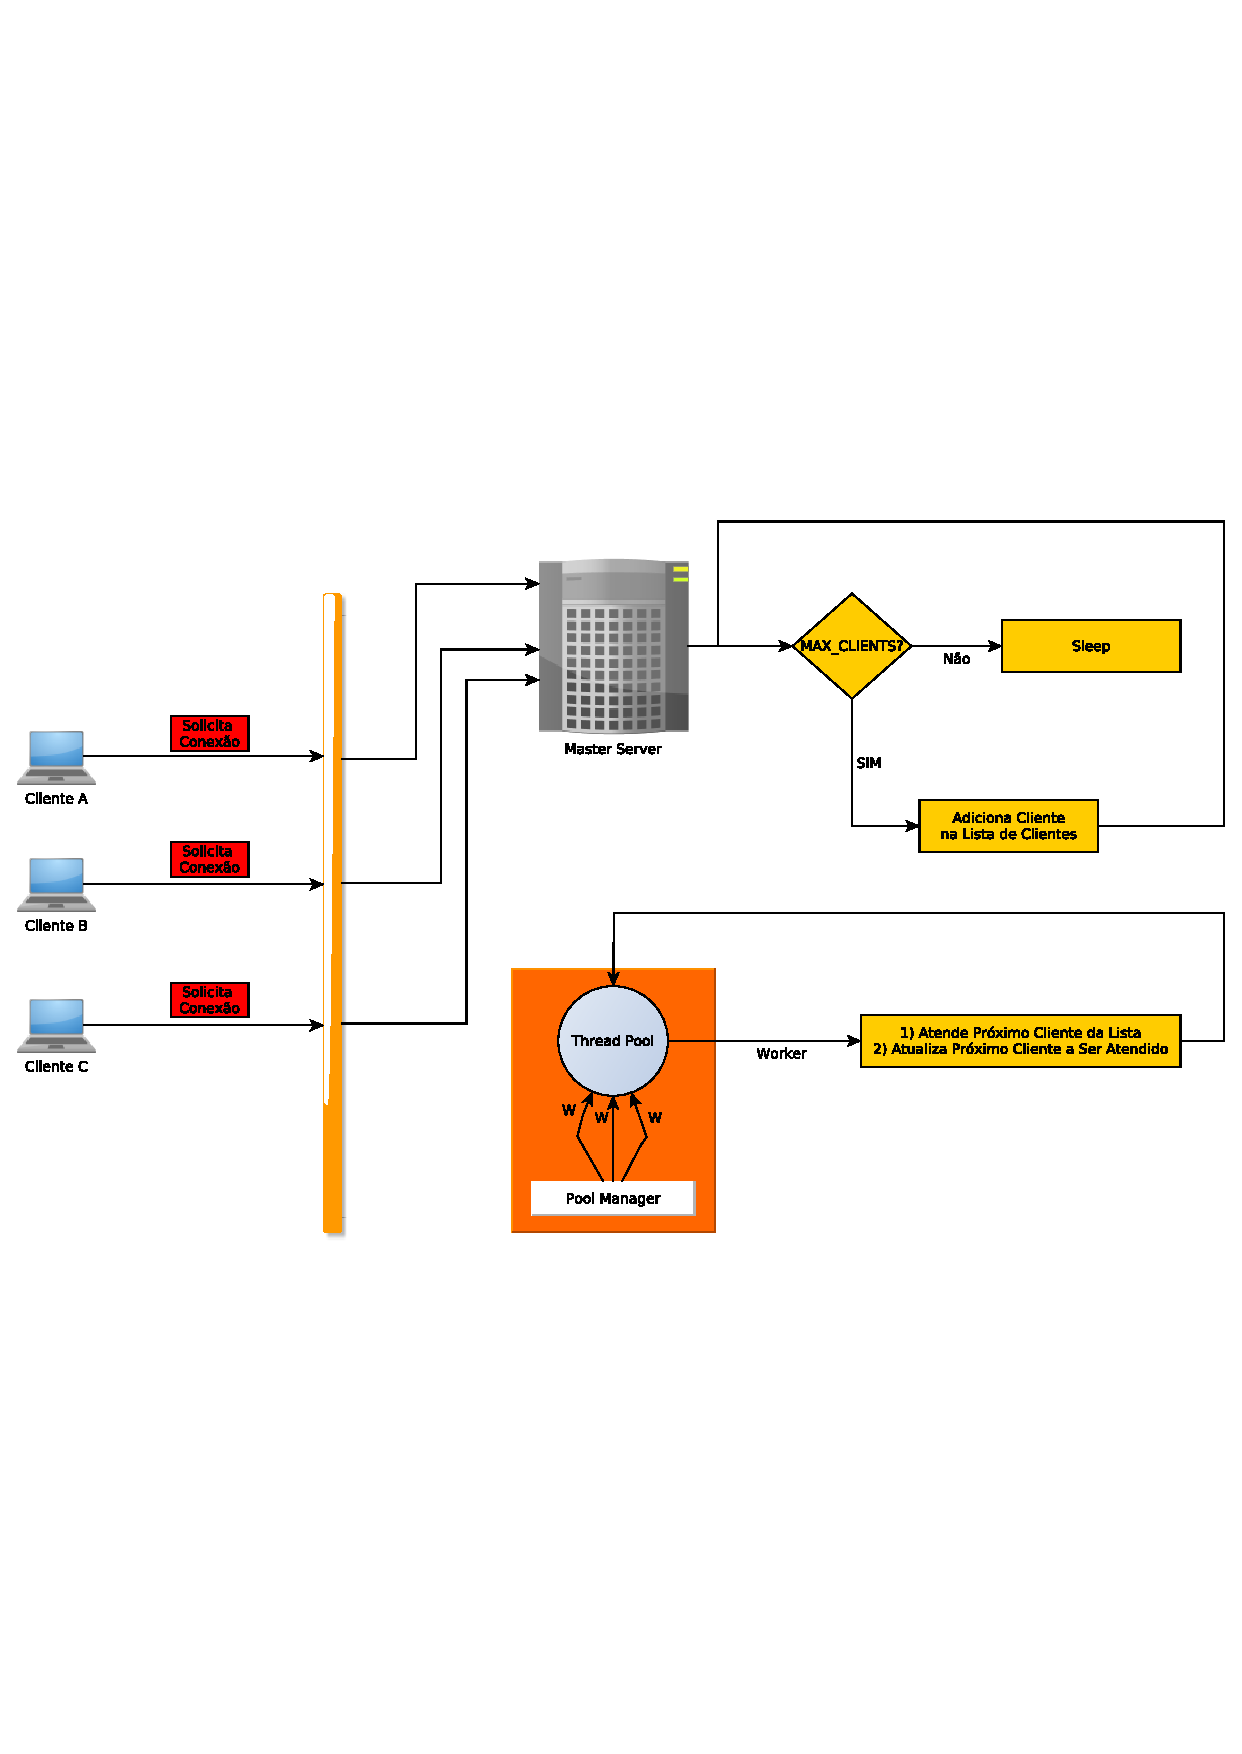
\includegraphics[clip,trim=0cm 5.5cm 0cm 5.5cm,width=1\textheight]{Img/AppSchematic}
	\end{sidewaysfigure}

\clearpage
\section{Manual do cliente\label{app:manC}}

\begin{lstlisting}

************************************************************
Y A S C  --  ClientHelpFile   [Revision 2]
************************************************************

=== Calling Procedure ===

  ./yascC.exe <hostname> <port>
    It is suggested to run from within directory ./program/.
    Use 'make runC' after changing the arguments to avoid writing the arguments all the time.

  Options:

  -g              start in debug mode

  -f <file.txt>   takes commands from file.txt instead of command line
                  (.txt extension not enforced)

  -l              creates log.txt and runs silently
                  (Critical errors are still posted on the command line rather than the log file)


=== Syntax ===

  Interpreter:
    The parsing function only takes into account blocks of characters separated by white space.

  Numbers:
    1) have to be integers
    2) shall not be preceded by 'D'
    3) may have an extra attribute, the signal, in the format '-###' or '+###' without spaces
    4) may be given in decimal format as '###'; hexadecimal as '0x###' or octal as '0###'

  Math:
    Server uses Reverse Polish Notation.
    Any inconformity will result in unwanted behaviour, with or without errors, depending on mathematical correctness.

  Special cases:
    ';' marks EVERYTHING written afterwards in the same line as comments to be discarded.

    In a command file, every command is issued as soon as it is read, so EXIT marks the end of the program
    regardless of any command or random text that comes afterwards.


=== Commands ===

  'I'                   Begins session: connection is established; server issues a stack.
                        Server cleans the stack if there is one already.

  'K'                   Ends session: server erases stack; connection is terminated. Returns nothing.

  'P'                   Asks server for the stack size. Always succeeds.

  'T'                   Asks server for the top most value in the stack.

  'R'                   Asks server for end result; cleans the stack only if there is one value in the stack.
                        If the result is a partial one (i.e. there are still values in the stack), or if the stack is empty,
                        the server shall return an error. To see partial results use 'T'.
                        In case of error, returns BIG_STACK or BAD_STACK.

  'G'                   Sets debug flag for extra output.

  '+','-','*','/','%'   Integer basic operations. In case of error, return OUT_OF_RANGE, and also DIV_0 for '/' and '%'.

  'D' [deprecated]      Command is still issued internally whenever a number is found; direct usage results in parsing error.
                        Doesn't break the flow of the program, nor it is checked for good use (i.e. right before a number).

  'HELP'                Opens *this* document on the standard output, even if the -l flag is set.

  'EXIT'                Exits the program without prompt.


=== Output ===

  There are three kinds of output:

    >>       Internal errors that break functionality of the client; doesn't get redirected or suppressed with any flag.
             Program always exits after one of these.

    ::       Normal output; includes minor internal errors, and external errors (i.e. server errors); gets redirected with -l flag.

    DEBUG:   Additional / alternate output; present when -g flag is set or 'G' issued; gets redirected with -l flag.


=== ERROR codes ===

  These codes are defined in globalHeader.h.

  OUT_OF_RANGE      Over/Underflow; arithmetic result is out of range (min/max range defined as INT_MIN/INT_MAX in limits.h).
  DIV_0             Division by 0 detected.
  BIG_STACK         Stack is bigger than expected for specified operation.
  BAD_STACK         Not enough operands for specified action.



(SCROLL UP ^)
************************************************************

\end{lstlisting}

\clearpage
\section{Manual do servidor\label{app:manS}}

\begin{lstlisting}

************************************************************
Y A S C  --  ServerHelpFile   [Revision 1]
************************************************************

=== Calling Procedure ===

  ./yascS.exe <port>
    It is suggested to run from within directory ./program/.
    Use 'make runS' after changing the arguments to avoid writing the arguments all the time.

  Options:

  -v            verbose mode


=== Syntax ===

  Interpreter:
    The parsing function only takes into account commands separated by white space.


=== Commands ===

  'M'                   Prints information about every client logged on the server.
                        Format is: <IP address> [ stack element 1, stack element 2, ... ].

  'V'                   Verbose mode.

  'HELP'                Opens *this* document on the standard output.

  'F'                   Exits the program without prompt.


=== Services ===

  All communications shall use a package of 9 bytes.
  The first one is a message: 'V', 'E' or 'I'.
  The second one is an integer in hexadecimal format.


  Calculator:

    This server deploys a threaded fully compliant integer calculator with correct handling of mathematical / computational exceptions.
    For each correctly handled command, it shall return a message 'V' and a number, being 0 for padding, and a numerical result for relevant commands.

    The calculator interface is possible through a socket in the following format:

      'I'                   Begins session: connection is established and a stack is issued.
                            The server cleans the stack if there is one already.

      'K'                   Ends session: stack is erased; connection is terminated. Returns nothing to the client.

      'P'                   Returns the stack size. Always succeeds.

      'T'                   Returns the top most value in the stack.

      'R'                   Returns end result and cleans the stack only if there is one value in the stack.
                            If the result is a partial one (i.e. there are still values in the stack), or if the stack is empty,
                            the server shall return an error. To see partial results use 'T'!
                            In case of error, returns BIG_STACK or BAD_STACK.

      '+','-','*','/','%'   Integer basic operations. In case of error, returns OUT_OF_RANGE, and also DIV_0 for '/' and '%'.

      'D hex number'        Hexadecimal number is converted to integer and stored in the client's stack.


  Error codes:

    The server shall return these codes, defined in globalHeader.h, alongside with a message 'E' in case of ill usage:

    BAD_CMD           Nonconforming message received.
    OUT_OF_RANGE      Over/Underflow; arithmetic result is out of range (min/max range defined as INT_MIN/INT_MAX in limits.h).
    DIV_0             Division by 0 detected.
    BIG_STACK         Stack is bigger than expected for specified operation.
    BAD_STACK         Not enough operands for specified action.

    The server shall return these codes, defined in globalHeader.h, alongside with a message 'I' in case of internal error:

    [none defined]


=== Output ===

  There are three kinds of output:

    >>       Internal errors that break functionality of the server. Program always exits after one of these.

    ::       Normal output; includes minor internal errors.

            'M' command has a specific printing layout already covered above.


(SCROLL UP ^)
************************************************************

\end{lstlisting}